\chapter{Robert - \emph{Spell checking}}

Robert est un module capable de détecter le langage utilisé dans un texte donné, et éventuellement
 indiquer à l'utilisateur les différentes fautes que peut contenir ledit document en lui donnant une
sélection de mots considérés comme étant probables.  

\section{Génération des Dictionnaires}
Un dictionnaire est un fichier contenant un ensemble de mots, appartenant à une langue spécifique,
que l'on peut retrouver dans un texte.\\
Nous ne les avons pas généré, c'est un travail bien trop fastidieux, d'autant plus qu'il est aisé d'en
trouver sur Internet, sous la forme de fichier texte doté d'un mot par ligne ; Par exemple, un dictionnaire
anglais ne contient pas moins de 150 000 mots, et le dictionnaire français passe la barre des 700 000.
Seulement, si à chaque fois que l'on souhaitait vérifier l'existence d'un mot dans une langue donnée, il
faille parcourir les 700 000 lignes du fichier de manière séquentielle, le temps pris risque d'être énorme,
d'autant plus qu'un texte n'est généralement pas composé d'un seul mot, mais de plusieurs centaines, voir des
milliers. C'est pourquoi nous effectuons un prétraitement lors de l'ajout d'une langue à Robert : il s'agit
de la génération d'une structure de données au temps de recherche constant contenant l'ensemble des mots
appartenant à la langue donnée : La table de hashage, ou hashtable s'est donc imposée par défaut, grâce à
son temps de recherche constant, quelque soit la taille de l'ensemble qu'elle contient. \\
Ainsi, lors du chargement de Robert, OCaml va générer à partir des fichiers dictionnaires de chaque langue
reconnue des nouveaux dictionnaires (qui sont des hashtable)  reconnaissant la langue en RAM. \\
Un dernier soucis reste que la génération de ces dictionnaires nécéssitent obligatoirement une lecture
séquentielle de la hashtable, ainsi qu'un certain nombre de calculs quant à leur générations. \\Au final,
le chargement entier de la table de hash à partir du fichier texte ne prend pas moins de 1 seconde par langage.
Dans le doute, si jamais Robert devait être capable de gérer plusieurs dizaines de langages, le programme prendrait
pas moins de plusieurs dizains de secondes, rien qu'au chargement du module.

La solution a été trouvée grâce au module Marshall D'OCaml, qui permet de sérialiser un object en un tableau de bytes,
c'est à dire de copier sa représentation RAM dans un tableau de byte, et inversement. L'intérêt majeur est qu'il s'agit
d'une opération peu chère, qui permet de sauvegarder alors ce tableau dans un fichier binaire, pour le recharger
éventuellement plus tard. La génération du dictionnaire à partir du fichier source n'a alors à être réalisée qu'une
seule et unique fois par les développeurs, et Robert chargera et désérializera alors les dictionnaires à chaque fois
où KibiOCR sera appelé. Le gain apporté est assez conséquent, étant donné que l'on peut constater d'une ammélioration
de vitesse approchant les 1 000\%

\section{Détection d'un langage dans un texte donné}
L'algorithme de détection de langage actuellement utilisé est assez simple et redoutable d'efficacité :\\
Il analyse les X premiers mots (ou moins si le texte en fait moins) du texte qu'on lui donnera ; pour chaque langage, il contera alors le nombre de mots
reconnus. Une fois au les X mots traités, le langage retenu par la détection sera alors celui ayant le plus de termes reconnus.\\
\\
La constante X a été définie à 200, ce qui reste un nombre raisonnable du point de vue temps pris, tout en permettant de passer outre les
éventuelles erreurs que le texte peut comporter.\\
\section{Détection des termes incorrects}
La démarche utilisée est à peu près similaire ; robert va lire mot par mot l'ensemble du texte. A chaque fois qu'un mot n'existe pas dans le dictionnaire,
Robert va alors chercher quels mots pourraient correspondre. 
\section{Sélection des corrections possibles}
Généralement, quand un mot est incorrect, c'est que l'utilisateur l'ayant tapé l'a avant tout pensé phonétiquement, et a donc écrit correctement le mot,
phonétiquement parlant. Ainsi, "partez", qui est correct, peut devenir "parté", qui lui est incorrect.\\
Le système de correction orthographique de Robert a été pensé pour palier à cette déficience humaine, qui tend à empirer de nos jours...\\
C'est pourquoi nous avont implémenté en tout premier lieu l'algorithme phonétique Soundex, qui permet de générer une chaine phonétique à partir de n'importe
quel mot, à condition de connaître la langue auquel il appartient, étant donné que les prononciations varient sensiblement d'une langue à une autre, par exemple
entre le marseillais et le ch'ti.
L'algorithme se base sur le fait que ce qui permet d'identifier la prononciation phonétique d'un mot, ce ne sont pas les voyelles, mais au contraires les consonnes ;
Il va donc éliminer dans un premier temps toutes les voyelles du mot. Ensuite, les consonnes sont associées à un groupe donné, et remplacées par le chiffre correspondant :\\
\begin{itemize}
	\item 1 = B, P
	\item 2 = C, K, Q
	\item 3 = D, T
	\item 4 = L
	\item 5 = M, N
	\item 6 = R
	\item 7 = G, J
	\item 8 = X, Z
	\item 9 = F, V
\end{itemize}
Cette liste de groupes correspond à la pronciation français, il va de soi que pour l'anglais, elle varie: \\
\begin{itemize}
	\item 1 = B, F, P, V
	\item 2 = C, G, J, K, Q, S, X, Z
	\item 3 = D, T
	\item 4 = L
	\item 5 = M, N
	\item 6 = R
\end{itemize}
Ensuite, toutes les redondances de chiffres (par exemple P suivi de F donnera 11 en anglais, ce qui est une redondance) sont réduites à un seule chiffre,
et la chaîne de caractères ainsi obtenue est une chaîne phonétique Soundex.\\
Maintenant que l'on sait si deux mots donnés sont phonétiquement équivalents, il faut être capable de trouver l'ensemble des mots équivalents ; c'est 
pourquoi nous allons encore une fois passer par les merveilleuses table de hashage, afin de générer un dictionnaire phonétique.\\
Avant la mise en production, différents dictionnaires phonétiques sont générés en fonction des langues, qui à une chaîne soundex donnée, renvoient
 une liste contenant tous les mots équivalents. 
Seulement, il arrive que plusieurs dizaines de mots puissent être proposés, et afin d'éviter que l'utilisateur se perde (se noie) dans le flot de propositions,
il est impératif de trier l'ensemble, afin de sortir uniquement les X termes jugés les plus pertinants. Il est évident que si un mot fait 6 lettres, il est inutile
de proposer des choix de 42 lettres, les probabilités que l'utilisateur aie voulu taper le mot de 42 lettres étant malheureusement trop faibles.\\
C'est pourquoi un deuxième algorithme intervient alors, qui mesure la distance d'édition entre deux mots, c'est à dire qui mesure le nombre minimal d'opérations élémentaires
(déletion, ajout, remplacement) nécéssaires afin de transformer un mot A en un mot B. Cet algorithme est la "distance de Levenshtein".\\
La liste totale des éventuelles propositions est alors triée par ordre croissant en fonction de la distance de levenshtein entre chaque mot de la liste et le mot originel incorrect,
et seuls les X premiers termes de la liste sont alors retenus, X ayant été choisi par défaut comme étant 5.
Robert permet ainsi une proposition de correction orthographique puissante.
\begin{center}
	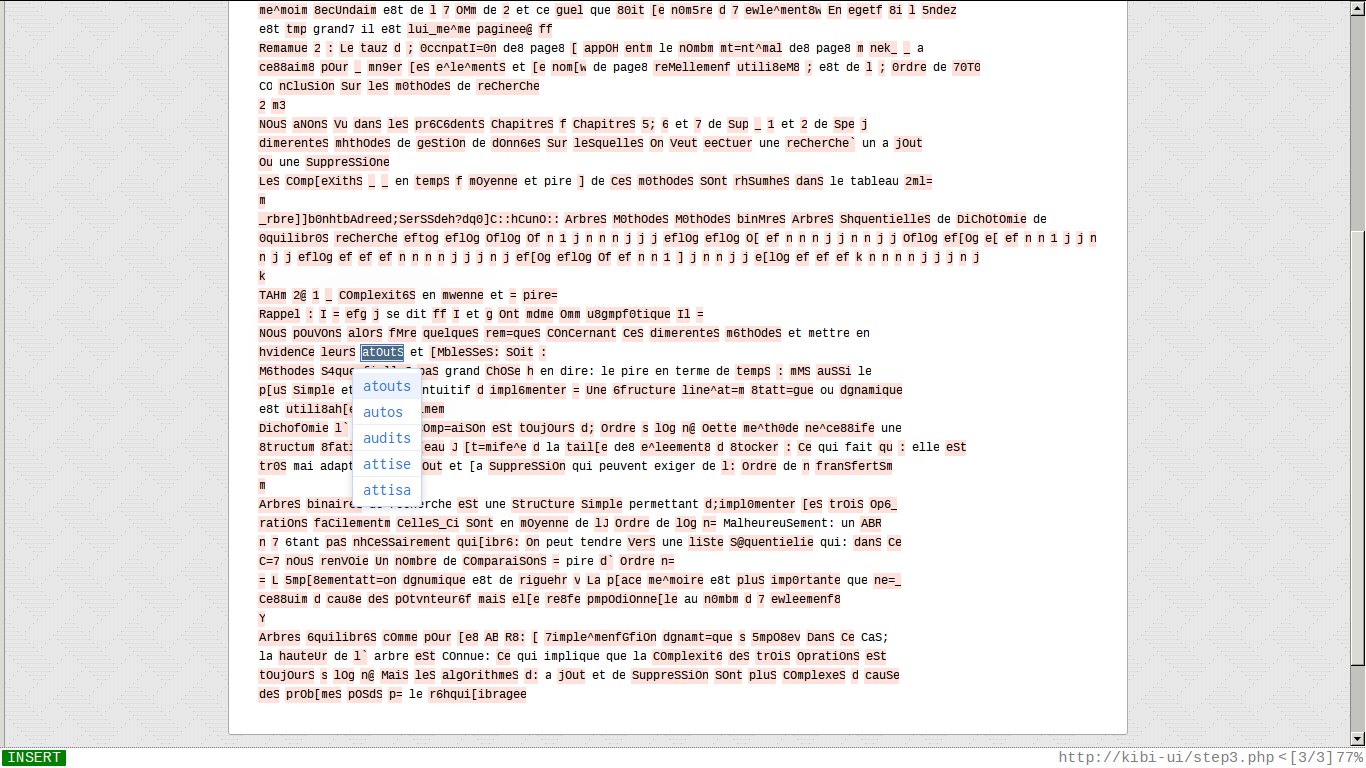
\includegraphics[scale=1]{Pictures/robert.png}
	\caption{Notre bon vieux Robert à l'action}
\end{center}
